\documentclass[tikz,border=5mm]{standalone}
\usepackage{tikz}
\usetikzlibrary{arrows.meta, positioning, shapes.geometric, calc, backgrounds, fit, matrix, patterns}

% --- COLOR DEFINITIONS ---
\definecolor{Garnet}{HTML}{73000A}
\definecolor{CSecondaryRed}{HTML}{CC2E40}
\definecolor{CBlue}{HTML}{466A9F}
\definecolor{CDark}{HTML}{1F414D}
\definecolor{COlive}{HTML}{65780B}
\definecolor{CLime}{HTML}{CED318}
\definecolor{CGold}{HTML}{A49137}
\definecolor{CGrayLight}{HTML}{E5E5E5}
\definecolor{CGrayDark}{HTML}{555555}

\begin{document}
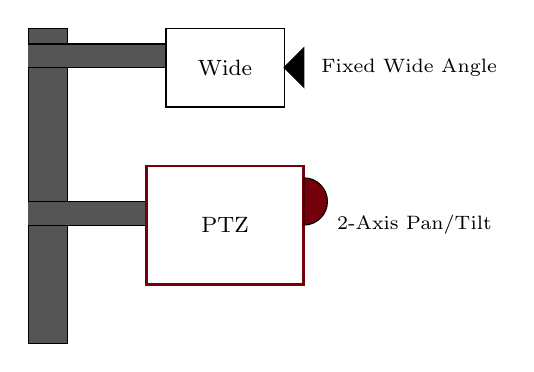
\begin{tikzpicture}
  % Mount
  \draw[fill=CGrayDark] (0,0) rectangle (0.5, 4);
  \draw[fill=CGrayDark] (0, 3.5) -- (2, 3.5) -- (2, 3.8) -- (0, 3.8);
  % Wide Camera
  \node[fill=white, draw=black, minimum width=1.5cm, minimum height=1cm, label={center:\footnotesize Wide}] (W) at (2.5, 3.5) {};
  \draw[fill=black] (3.25, 3.5) -- (3.5, 3.25) -- (3.5, 3.75) -- cycle; % Lens
  % PTZ Camera
  \draw[fill=CGrayDark] (0, 1.5) -- (2, 1.5) -- (2, 1.8) -- (0, 1.8);
  \node[fill=white, draw=Garnet, line width=1pt, minimum width=2cm, minimum height=1.5cm, label={center:\footnotesize PTZ}] (P) at (2.5, 1.5) {};
  \draw[fill=Garnet] (3.5, 1.5) arc (-90:90:0.3) -- cycle; % Dome lens rep
  % Labels
  \node[right, font=\scriptsize] at (3.6, 3.5) {Fixed Wide Angle};
  \node[right, font=\scriptsize] at (3.8, 1.5) {2-Axis Pan/Tilt};
\end{tikzpicture}
\end{document}
